% MAT E 374 group project: report template (ACS journal style, achemso class).
% Upload the distributed source ZIP to Overleaf. In the course checkout, compile with: latexmk -pdf report.tex
% The release builder inserts a bibliography copy from the root references.bib into that ZIP.
% Blue text is a placeholder: replace it with your own words, numbers, and figures,
% and remove \placeholder{} when you are done. The example figures are from the
% instructor's test runs; replace every figure with your own.
\documentclass[journal=jpccck,manuscript=article,layout=twocolumn]{achemso}

\usepackage{xcolor}
\usepackage{graphicx}
\usepackage{amsmath}
\usepackage{siunitx}
\newcommand{\placeholder}[1]{\textcolor{blue}{#1}}

\title{\placeholder{Size, Shape, and Heating Rate in the Simulated Melting of Copper Nanoparticles}}

\author{\placeholder{First Member}}
\author{\placeholder{Second Member}}
\author{\placeholder{Third Member}}
\author{\placeholder{Fourth Member}}
\author{\placeholder{Fifth Member}}
\affiliation{Department of Chemical and Materials Engineering, University of Alberta, Edmonton, Alberta, Canada}
\email{contact.member@ualberta.ca}

\begin{document}

\begin{abstract}
\placeholder{At most 200 words: question, method, main results. For example: We simulated the melting and freezing of free Cu nanoparticles 2--8~nm in diameter with
molecular dynamics and an embedded-atom potential. The melting temperature decreased from xxx~K at 8~nm
to xxx~K at 2~nm, and a fit of $T_\mathrm{m} = T_\mathrm{m,bulk} - C/D$ gave $T_\mathrm{m,bulk} = $ xxx~K.
Particle shape changed the melting temperature by up to xxx~K, while a faster heating rate raised it by
xxx~K. The particles froze xxx~K below their melting point. We conclude that yyy.}
\end{abstract}

\section{Introduction}
\placeholder{Why does nanoparticle melting matter? Give one or two applications and cite them. Summarize what is known: small particles melt below the
bulk melting point~\cite{buffat1976gold}, and this melting point depression follows approximately
$T_\mathrm{m}(D) = T_\mathrm{m,bulk}[1-(D_0/D)^{\alpha}]$.}

\placeholder{End with the questions of this work: the effects of size, shape, and heating rate, which are
physical, and what a fit tells us about bulk copper.}

\section{Methods}
\placeholder{Give enough detail that another group could repeat your work. For example: The atoms interacted through the embedded-atom method (EAM) potential for Cu of Mishin
et al.~\cite{mishin2001cu}. Particles were built with the Atomic Simulation Environment
(ASE)~\cite{larsen2017ase} in xxx shapes and xxx diameters, without periodic boundaries. Molecular
dynamics was run in OpenMM~\cite{eastman2024openmm} with a Langevin thermostat (friction xxx~ps$^{-1}$)
and a time step of xxx~fs.}

\placeholder{List the temperatures, run lengths, heating rates, and number of seeds. State exactly how you
obtained each melting and freezing temperature, for example from the steepest rise of the energy or from the
fraction of crystal-like atoms~\cite{steinhardt1983bond}. Describe your own fitted potential here if you did
the bonus.}

\section{Results and Discussion}
\subsection{Equilibration}
\placeholder{Figure~\ref{fig:stability} shows that the potential and kinetic energies become stable
after about xxx~ps at xxx~K. The mean kinetic energy, xxx~eV per atom, agrees with
$\tfrac32 k_\mathrm{B}T = $ xxx~eV per atom within xxx\%. Close to the melting point, yyy.}

\begin{figure}[!htb]
  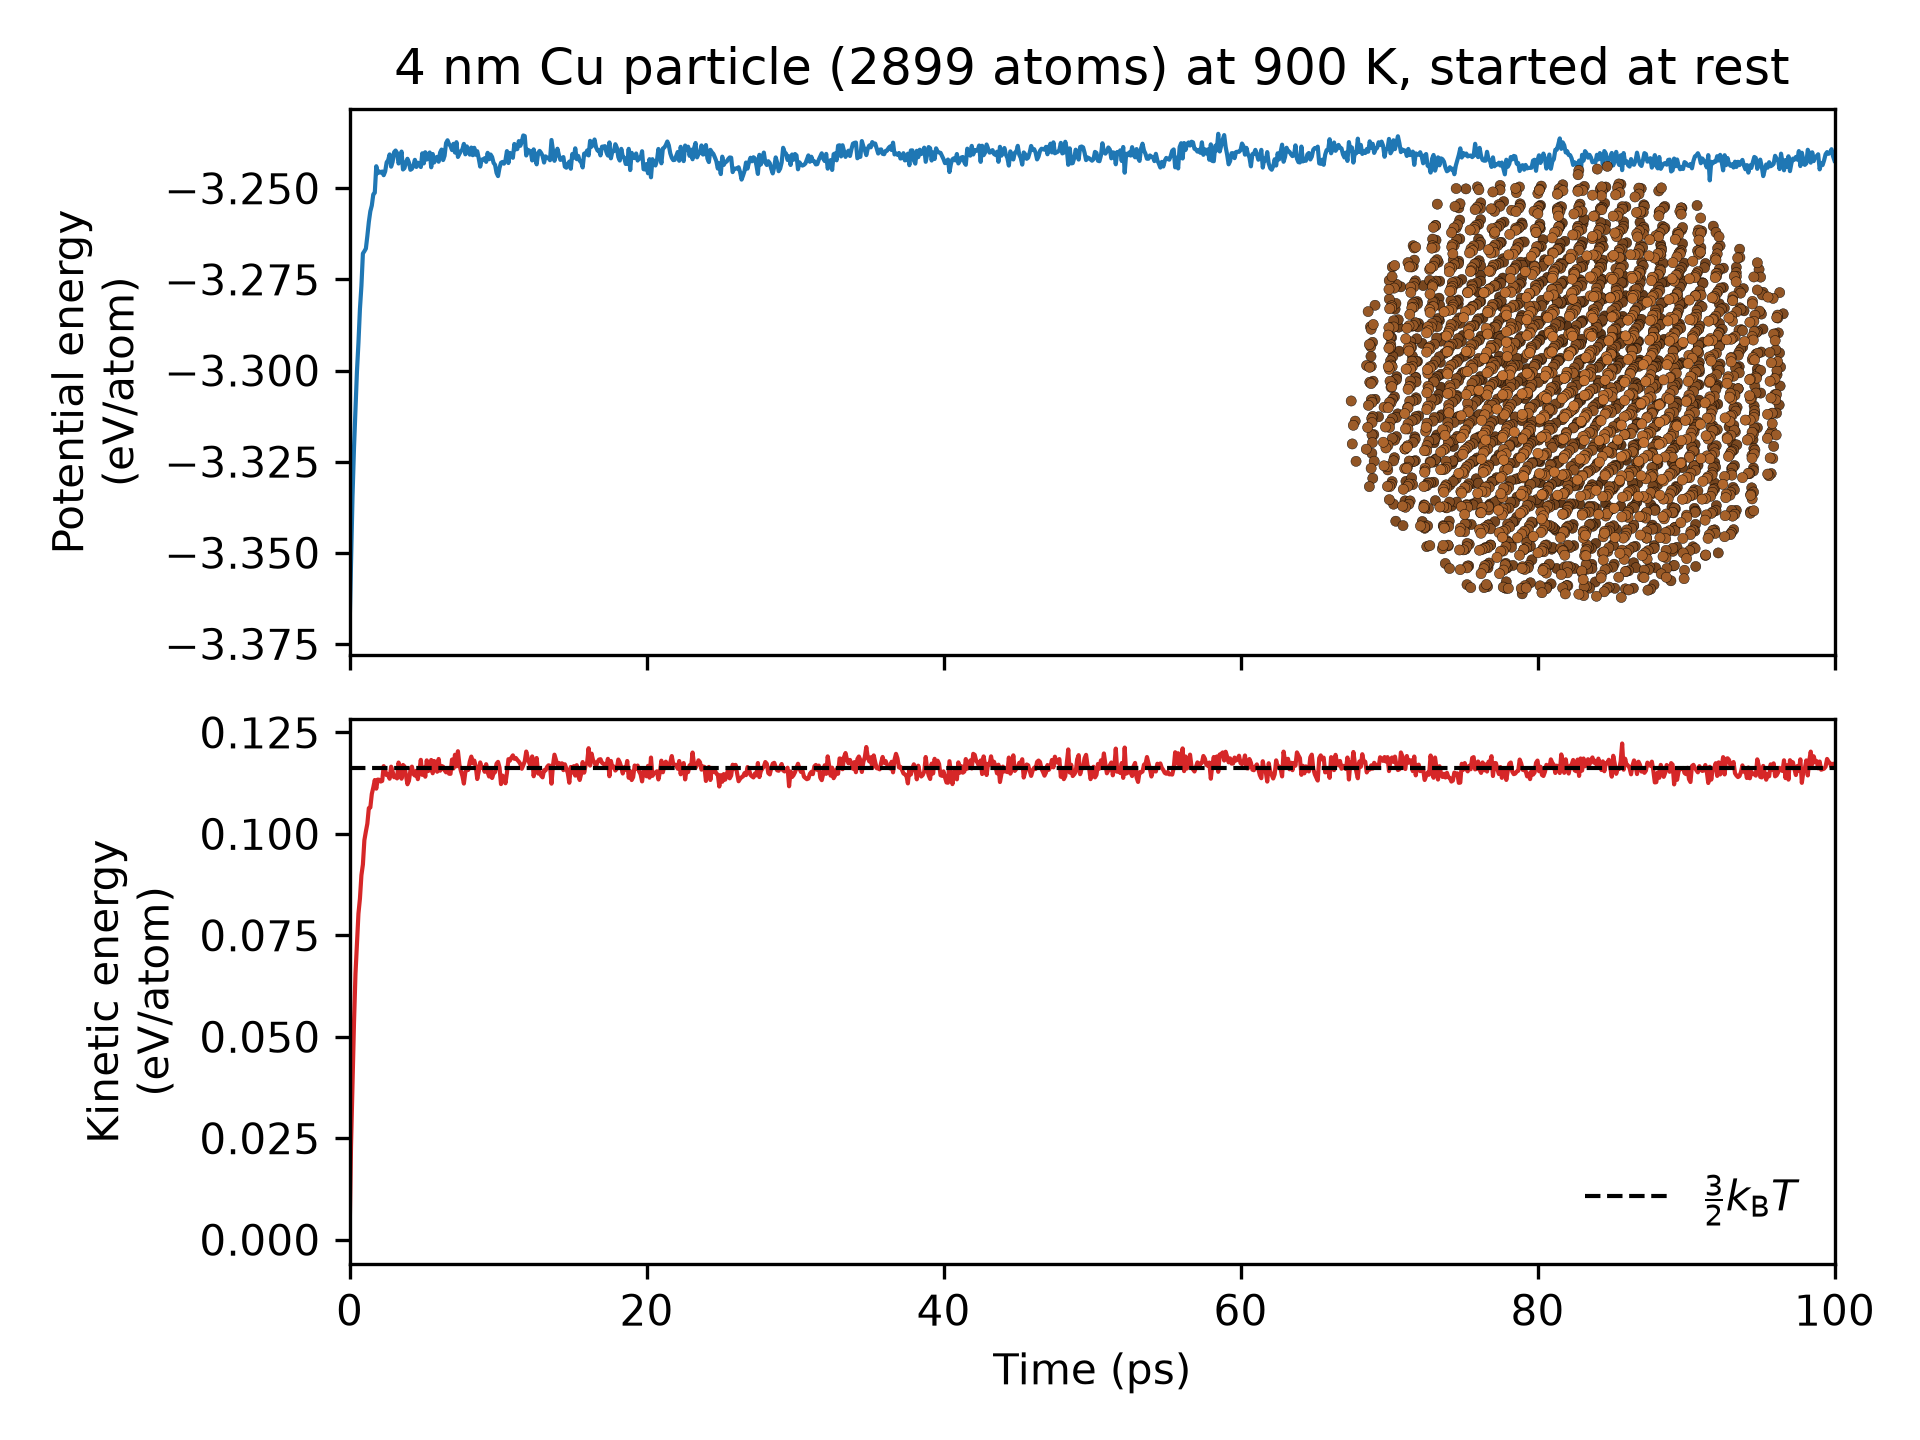
\includegraphics[width=\columnwidth]{fig_stability.png}
  \caption{\placeholder{Example figure. Potential and kinetic energy of a 4~nm particle (2899 atoms) at
  900~K, starting from the perfect crystal with all atoms at rest. Replace with your own figure and
  describe what it shows.}}
  \label{fig:stability}
\end{figure}

\subsection{Melting and Freezing}
\placeholder{Our simulations show a large difference between the melting and freezing temperatures in
the heating and cooling cycle (Figure~\ref{fig:cycle}). The particle melts at xxx~$\pm$~xxx~K but freezes
only at xxx~$\pm$~xxx~K. This corresponds to the phenomenon described by [author, year] as
[name of the effect]. Add the reference that supports your explanation. It occurs because yyy.}

\begin{figure}[!htb]
  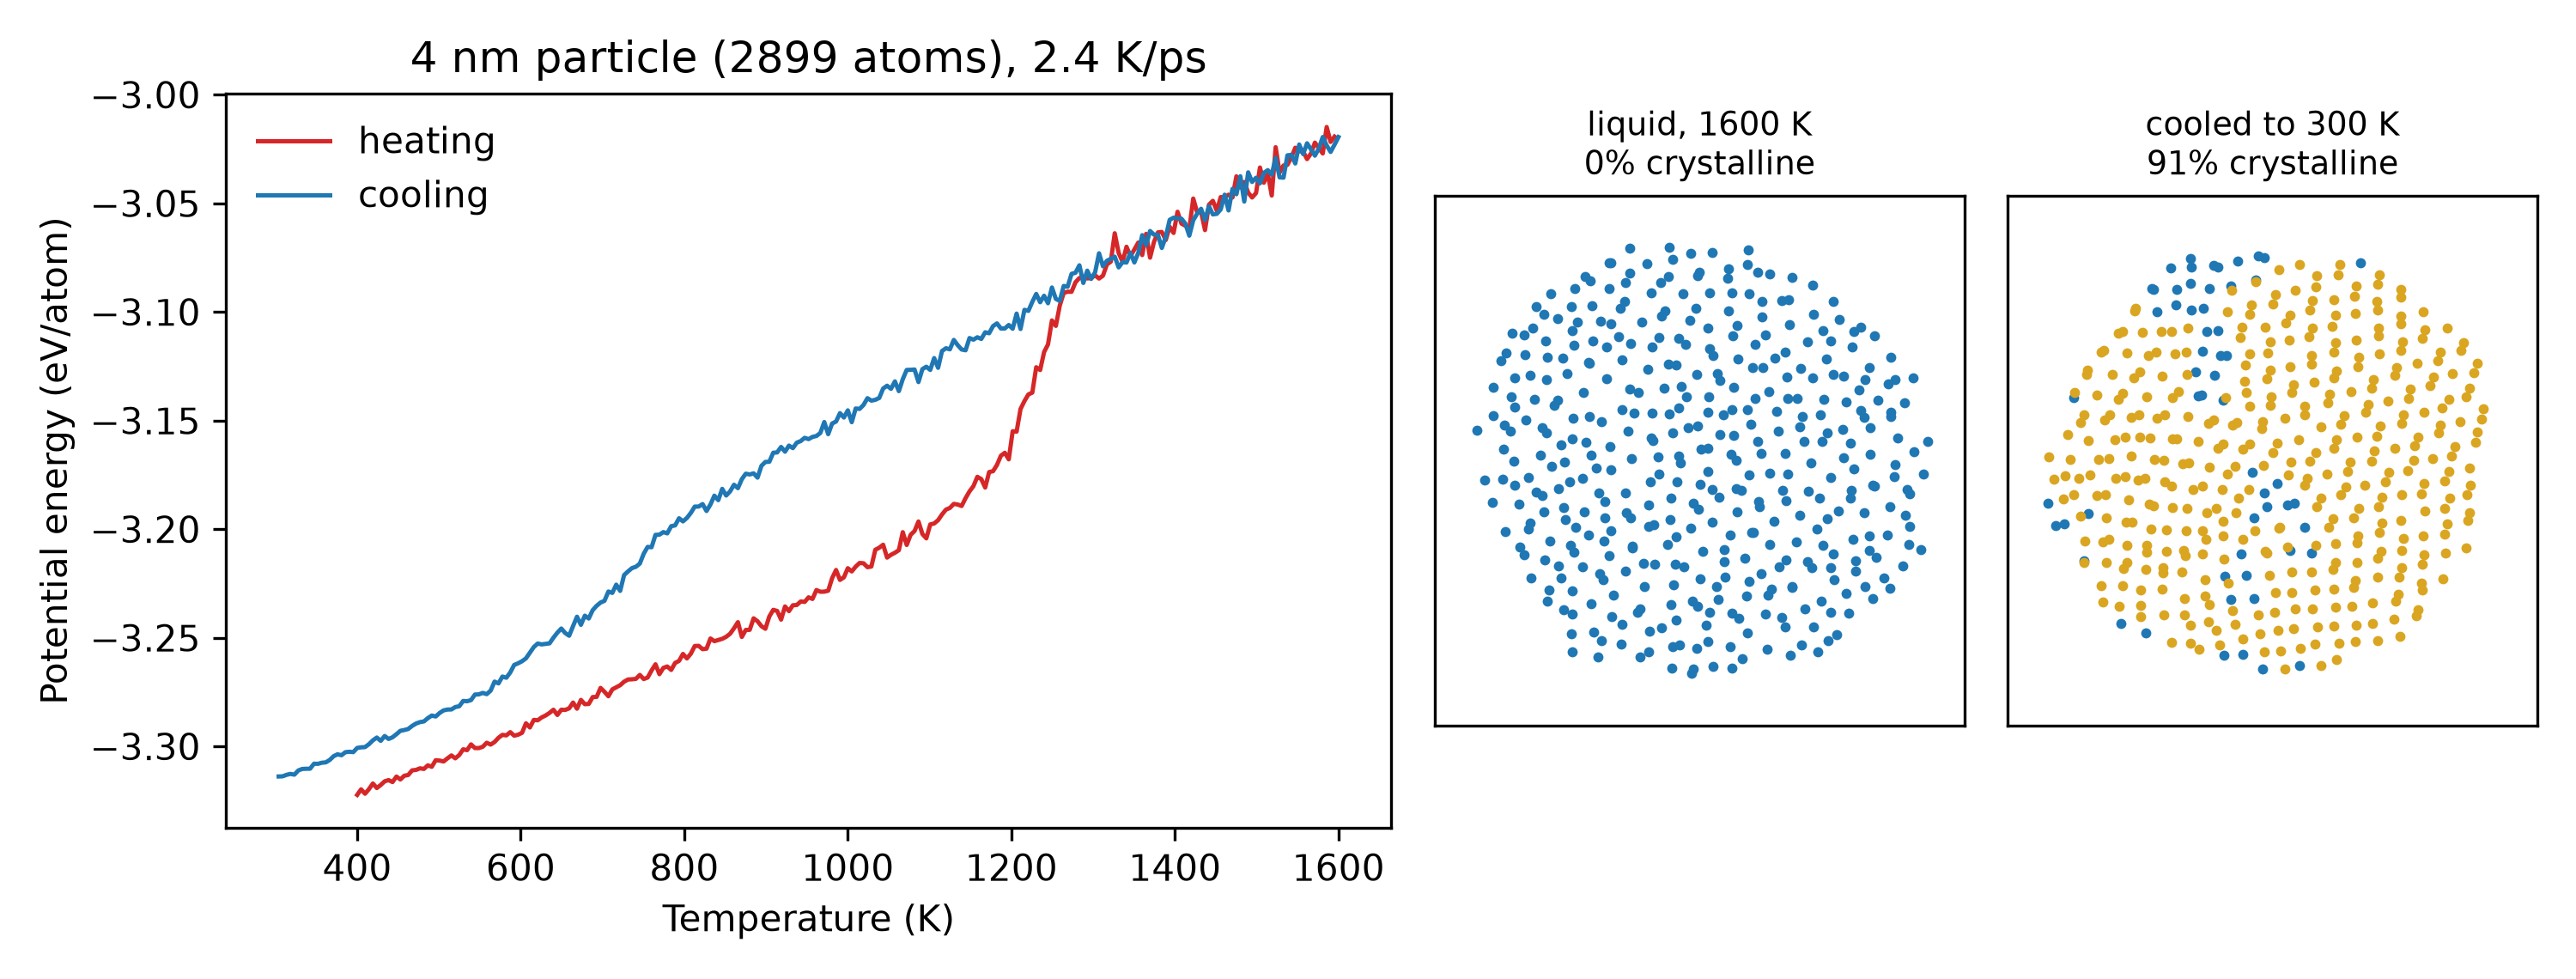
\includegraphics[width=\columnwidth]{fig_cycle.png}
  \caption{\placeholder{Example figure. Left: potential energy of a 4~nm particle heated and cooled at
  2.4~K/ps. Right: slices through the centre of the particle; gold atoms are crystal-like and blue atoms
  are liquid-like. Replace with your own figure.}}
  \label{fig:cycle}
\end{figure}

\subsection{Effects of Size, Shape, and Heating Rate}
\placeholder{Compare each effect with the scatter between repeated runs (xxx~K). Changing the diameter
from xxx to xxx~nm lowers the melting temperature by xxx~K. Changing the shape from xxx to xxx changes it
by xxx~K, which we attribute to yyy. A faster heating rate raises the measured melting temperature by xxx~K,
which indicates that zzz. Use a table if it is clearer than text.}

\subsection{Fit of the Size Dependence}
\placeholder{From our fitted curve (Figure~\ref{fig:size}) we obtained $T_\mathrm{m,bulk} = $ xxx~K and
$C = $ xxx~K\,nm, with uncertainties of xxx. Values of $\alpha$ between xxx and xxx are consistent with our
data, indicating yyy. The bulk value differs from the experimental melting point of Cu, 1357.77~K, by xxx~K because
zzz. Our experiments with zzz showed that changing the potential (or the heating rate) has an effect of
xxx~K.}

\begin{figure}[!htb]
  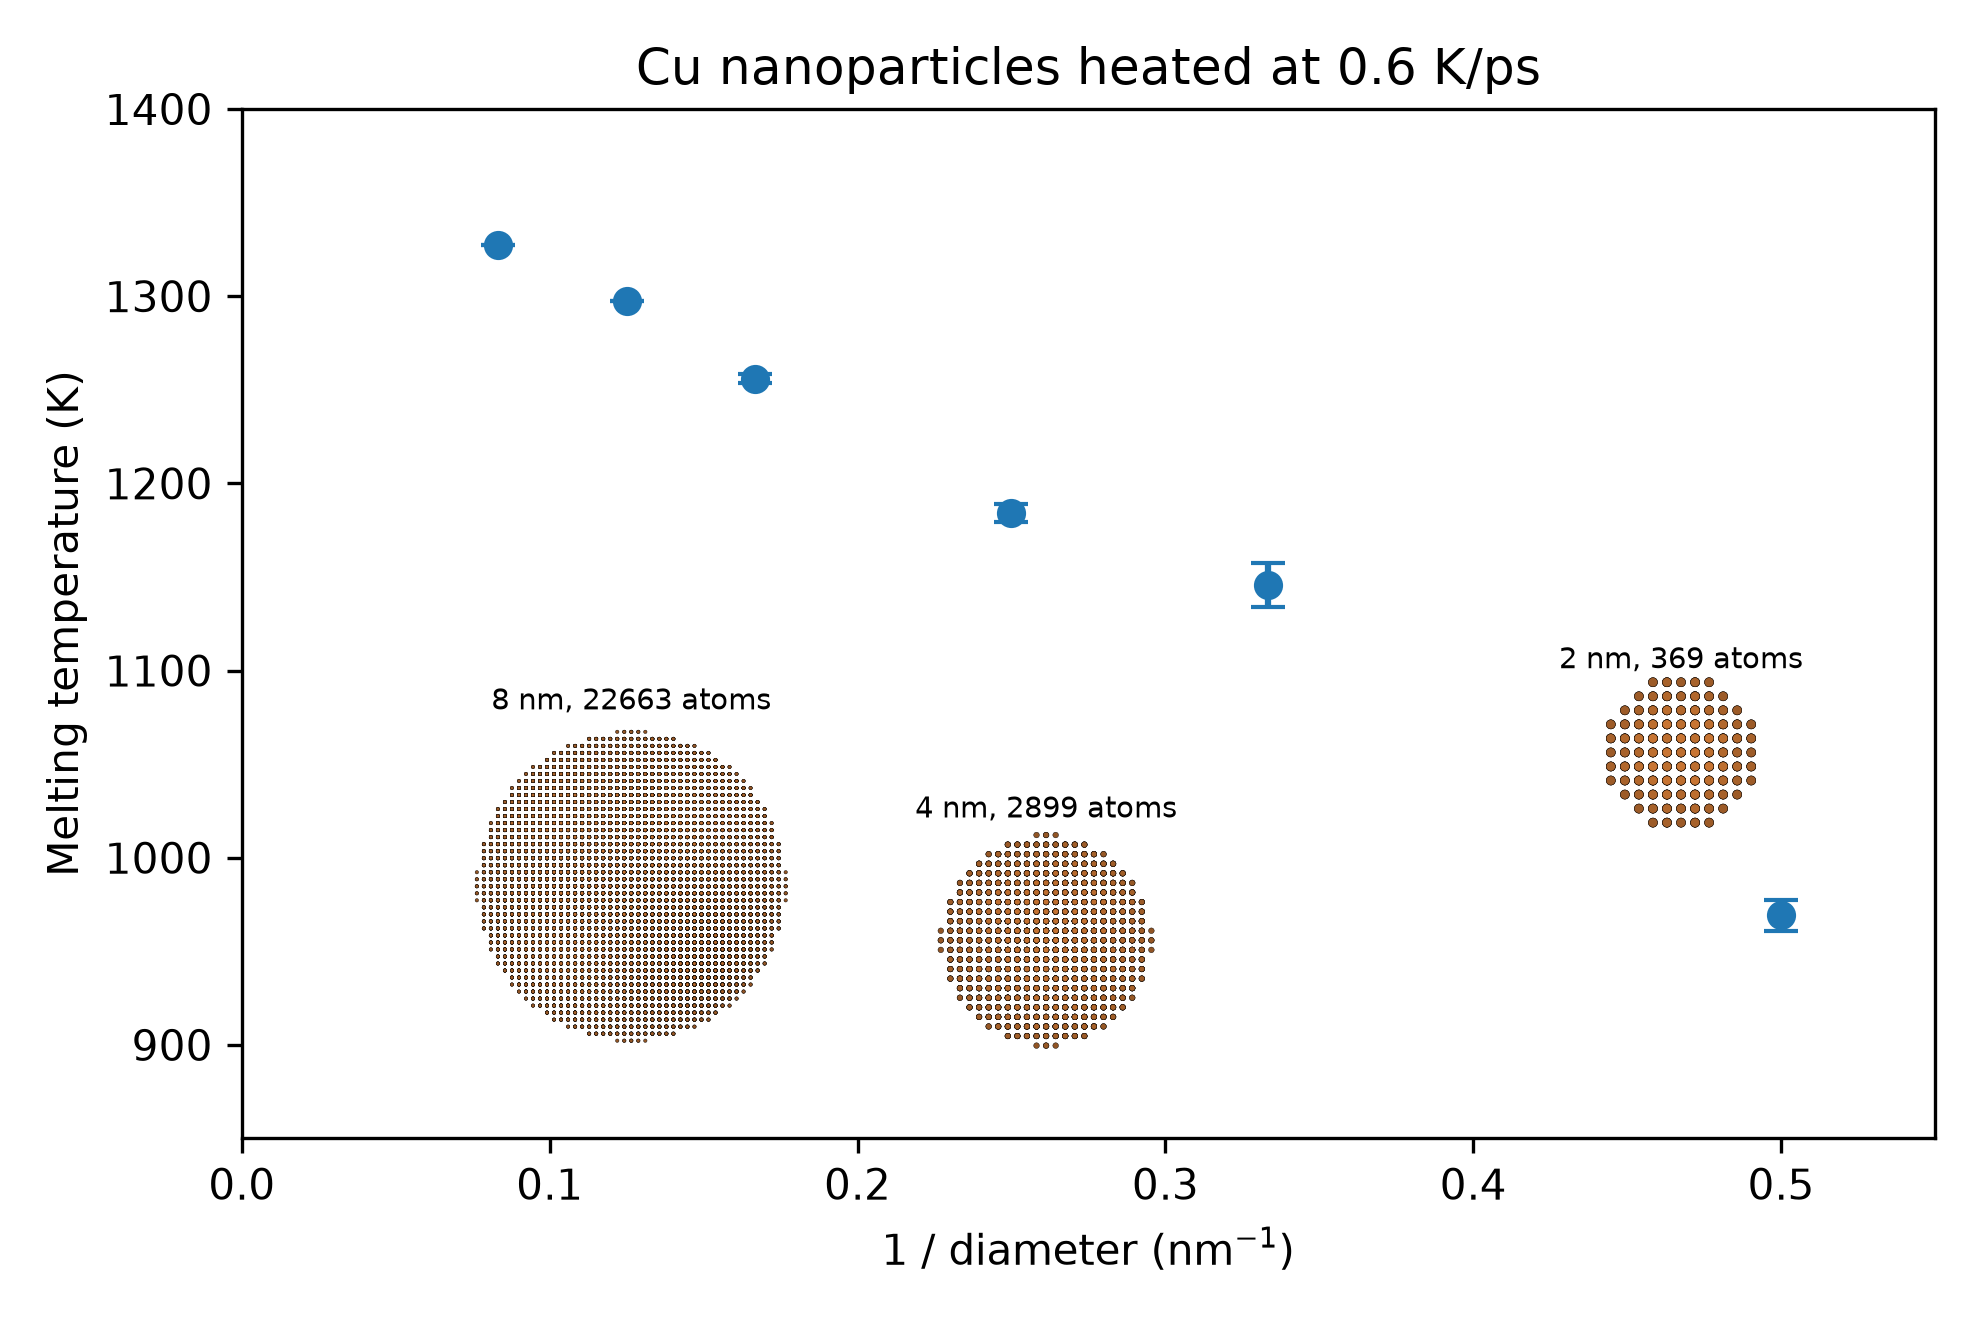
\includegraphics[width=0.9\columnwidth]{fig_size.png}
  \caption{\placeholder{Example figure. Melting temperature against inverse diameter, mean and spread of
  three runs. Replace with your own figure, and show your fitted curve.}}
  \label{fig:size}
\end{figure}

\subsection{Suggested Improvements}
\placeholder{What would you change to obtain a more reliable melting temperature, and why? Support each
suggestion with your results.}

\section{Conclusions}
\placeholder{State the main findings in three to five sentences, with numbers. Answer the three central
questions of the project directly.}

\begin{acknowledgement}
\placeholder{Contributions: Member 1 ran xxx; Member 2 analysed xxx; \ldots\ Use of AI: we used
[tool] for [task], and we checked [how].}
\end{acknowledgement}

\section*{Supporting Information}
\placeholder{The \texttt{.zip} file of \texttt{.csv} results and the notebook sources or molab links for every notebook
used.}

\bibliography{../../references}

\end{document}
